\subsection{Limitations}
\label{sec:current-limitations}

% Short intro
Different sources of errors and potential improvements can be identified for improving the accuracy of the models.
This section discusses those errors and how improvements can be implemented.

\subsubsection{Impact of fixed failure threshold}
\label{sec:fixed-failure-threshold}

The simulation presented earlier (Fig. \ref{fig:reference_simu}) clearly showed that the fixed threshold is a major source of modelling error.
The problem was particularly clear for on the signal V\textsubscript{1p0}.

It seems that the failure criteria should not be used as output amplitude value, because it oversimplifies the waveform of the output.
This is illustrated by figure. \ref{fig:impact-single-failure-criteria}.
Any disturbance under the failure criteria is modeled as no disturbance.
This is the case even if the disturbance is just below the failure criteria, without crossing it.
On the contrary, any disturbance beyond the failure criteria uses the failure level for modeling.
The max value of the output may be much larger than the failure criteria, however, it will still be modeled as a square pulse of amplitude Vfail.

\begin{figure}[!h]
  \centering
  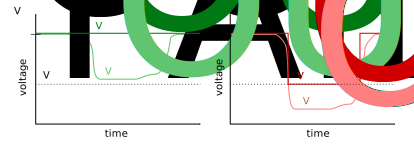
\includegraphics{src/4/figures/bad_output_modelling.pdf}
  \caption{Lack of accuracy caused by the use of a single failure criteria to model the output}
  \label{fig:impact-single-failure-criteria}
\end{figure}

% Remove failure criteria by table
In fact, the failure criteria itself

\subsubsection{Impact of characterization output load}

% First source of error - load impedance
Previously, all characterization curves were extracted with a fixed output load of 1M\textOmega{}.
This value was selected because it is rather high-impedance and does not prevent proper circuit operation.
It also draws a non-negligible amount of current and reproduces the circuit load of the complete schematic.
It is possible that this fixed high-impedance load is a factor of error for the model chain.

% Compare 1Mohm with real case where blocks are connected together
%TODO: Clarify
In practice, each block sees a load impedance on its output much different than 1 M\textOmega{}.
For instance, the output of the pre-regulator is used as a supply by other blocks.
It can deliver a maximum of 20 mA of current while maintaining 8V.
Thus, the minimum output load this block can sustain is 400 \textOmega{}.
The bandgap, on the other hand, provides a reference voltage at 1V but does not deliver a lot of DC current.
More than 1uA is enough to make the output fall of a hundred millivolts.
In this case, the bandgap must see an output impedance of at least 1 M\textOmega{}.

% What is done next
To evaluate this impact, the pre-regulator is characterized again by with 4 different load values ranging from 500 \textOmega{} to 1 M\textOmega{}.
Results are summarized in table \ref{tab:impact-load-on-cz}.
The three first column represent the input parameters, and the last column shows for how long the output was disturbed.
The duration is mesured using the failure criteria of the pre-regulator (V\textsubscript{clamp9} < 0V).
It is the time during which the failure criteria was violated.

% Table observation
For the smallest 10V stress amplitude, the failure time is largely impacted by the output load.
The worst case is for the -10V 1\textmugreek{}s pulse (Table \ref{tab:impact-load-on-cz}).
The output goes below 0V for 1330 ns with 500\textOmega{} on the output, but with 1M\textOmega{}, no failure is observed.
However, it is interesting to notice that for larger pulse amplitudes (below -30V), the output load has a limited impact on the failure duration.

% Analyse the table
Those observations tend to indicate that once the output is at fault, having 500\textOmega{} or 1M\textOmega{} connected to it doesn't change the period during which it remains at fault.
This is a major observation, because it shows that the output load value is not a key parameter during the characterization, and that the 1 M\textOmega{} value is sufficient for this study case.

\begin{table}[!p]
\centering
\begin{tabular}{llll}
\toprule
load (\textOmega) & amplitude (V) & length (ns) & output disturbed (ns)   \\ \midrule
500               & -10        & 10         & 10n    \\
5k                &            &            & 1n    \\
50k               &            &            & None    \\
1M                &            &            & None    \\
\rowcolor[gray]{.95}
500               &            & 100        & 100n    \\ \rowcolor[gray]{.95}
5k                &            &            & 1n    \\ \rowcolor[gray]{.95}
50k               &            &            & None    \\ \rowcolor[gray]{.95}
1M                &            &            & None    \\

500               &            & 1000       & 1330n    \\
5k                &            &            & 1289n    \\
50k               &            &            & None    \\
1M                &            &            & None     \\
\rowcolor[gray]{.95}
500               & -30        & 10         & 20n    \\ \rowcolor[gray]{.95}
5k                &            &            & 10n    \\ \rowcolor[gray]{.95}
50k               &            &            & 10n    \\ \rowcolor[gray]{.95}
1M                &            &            & 10n    \\

500               &            & 100        &  506n   \\
5k                &            &            &  580n   \\
50k               &            &            &  594n   \\
1M                &            &            &  594n   \\
\rowcolor[gray]{.95}
500               &            & 1000       & 2087    \\ \rowcolor[gray]{.95}
5k                &            &            & 2194    \\ \rowcolor[gray]{.95}
50k               &            &            & 2206    \\ \rowcolor[gray]{.95}
1M                &            &            & 2206    \\

500               & -45        & 10         & 46n    \\
5k                &            &            & 10n    \\
50k               &            &            & 10n    \\
1M                &            &            & 10n    \\
\rowcolor[gray]{.95}
500               &            & 100        & 657n    \\ \rowcolor[gray]{.95}
5k                &            &            & 715n    \\ \rowcolor[gray]{.95}
50k               &            &            & 717n    \\ \rowcolor[gray]{.95}
1M                &            &            & 727n    \\

500               &            & 1000       & 2668n    \\
5k                &            &            & 2764n   \\
50k               &            &            & 2800n    \\
1M                &            &            & 2800n    \\

\bottomrule
\end{tabular}
\caption{Impact of the output load on characterization results}
\label{tab:impact-load-on-cz}
\end{table}

% Visual explanation of why the impact of the load at small amplitude
Fig. \ref{fig:impact-time-domain-load} provides a visual representation of this observation, which is helpful for understanding this result.
When the output is disturbed and its amplitude is near the failure criteria, the load value has a strong impact on the width of the failure.
This is represented by the green curve in Fig. \ref{fig:impact-time-domain-load}.
A large load value such as 1 M\textOmega{} decreases the amplitude a little bit, causing the output to be above the failure criteria.
With 1 M\textOmega{}, no failure is recorded.
With a small load value (500 \textOmega{}) the output amplitude is increased a little bit (it becomes more negative).
This time, it is below the failure criteria and a failure is recorded.
This explains how the load has a large impact of the failure width for small stress amplitudes.

\begin{figure}[!h]
  \centering
  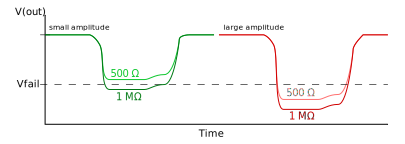
\includegraphics{src/4/figures/zout_impact_time_domain.pdf}
  \caption{Represented impact of output load impedance on the output waveform during a disturbance with a small amplitude (green) and a large amplitude (red)}
  \label{fig:impact-time-domain-load}
\end{figure}

% Explanation at large amplitude
For large stress amplitude (red curve of Fig. \ref{fig:impact-time-domain-load}), the amplitude variation caused by a 500 \textOmega{} load versus 1 M\textOmega{} is not sufficient to change the outcome.
In both cases, a failure will be recorded.

% Conclusion, the main impact is not the characterization load, but the single failure criteria
In conclusion, the load value used during characterization does not seem to be the main source of error.
Once again, it seems that a fixed failure criteria is a major issue and limiting factor.
It is responsible for the large variations observed in Table \ref{tab:impact-load-on-cz} at small amplitudes.
This results correlates with the observation made earlier in section \ref{sec:fixed-failure-threshold}, that also indicates that this fixed failure threshold should be removed.


\subsubsection{Impact of connections between blocks}
\label{sec:impact-missing-conns}

Failure signature is changed

Improvements are required

\subsubsection{Other sources}

%TODO: Make section ? Speak about limitations with multiples nets that are responsible for error propagation
%TODO: Limitation with multiple nets. Interactions between inputs. Diamond-like connections

% What was the promise of this model
This method looked rather promising in terms of applicability.
In theory, a block could be characterized once, and its model reused in different places.
The robustness of a full system could be quickly and easily deduced from the models of its parts.

% Real outcome is that it's not working well
However, with the study case exposed earlier, several issues arose that clearly limit the ability of the model to perform as expected.

% Main issue
So far the main issue of this method is to be limited to a binary fail/no fail criteria.
In some cases, the specification could be used to set this criteria, but mostly it was an arbitrary level.
For digital cells, a binary criteria is correct because above a certain input level disturbance an output can be switched, and the failure is then clear.
However, for most analog functions, there is no clear failure.
Most nets will have degraded values until extreme levels where biasing might completely fail.
Sometimes, the product is destroyed before reaching those extreme levels.
In any case, the binary criteria hides a lot of information about the degradation.

% Secondary issue
It was also suspected that the output load used during characterization might impact the results too much.
In practice, it was proven in the case of the regulator that this is not exactly true.
Changing the load can induce a varation, but seemingly more limited than the impact of the binary failure criteria.

% Directivity ?
% Basically : WE ASSUME STRESS AND FAILURES PROPAGATE FROM INPUT TO OUTPUT. MAY NOT BE THE CASE. ALSO, MAY NOT WORK IN REVERSE WITH SINGLE2MANY BLOCK CONNECTIONS

% Next
The next section will explore a modification of the characterization method to fix the binary failure criteria issue.
